\documentclass[12pt,a4paper]{article}
\usepackage{ngerman}
\usepackage[utf8]{inputenc}
\usepackage{sectsty, xcolor}
\usepackage{lastpage}
\usepackage{amsfonts, amssymb, array, enumitem, fancyhdr, graphicx, float, makeidx, textcomp, multicol, tabularx}
\usepackage[fleqn]{amsmath} %Math-Environment linksbündig
\usepackage{MnSymbol}
\usepackage[hidelinks]{hyperref}
\usepackage[hang,flushmargin]{footmisc}
\usepackage{tikz}

\newcolumntype{Y}{>{\centering\arraybackslash}X}

\setlist[itemize]{noitemsep,topsep=0pt,leftmargin=*}
\setlist[enumerate]{noitemsep,topsep=0pt,leftmargin=*}
\setlength\parindent{0pt}

\makeindex

% \definecolor{dunkelblau}{rgb}{0,0.4,0.6}
% \subsectionfont{\color{dunkelblau}}

\title{ANLIS HS 2020}
\author{Victor Fernández}
\date{}

\addtolength{\oddsidemargin}{-.875in}
\addtolength{\evensidemargin}{-.875in}
\addtolength{\textwidth}{1.75in}
\addtolength{\topmargin}{-.875in}
\addtolength{\textheight}{1.75in}

% muss nach Änderung der margin kommen!
\pagestyle{fancy}
\fancyhf{} %reset
\fancyhead[L]{HSLU}
\fancyhead[C]{ANLIS}
\fancyhead[R]{\thepage/\pageref{LastPage}}
\fancyfoot[L]{}
\fancyfoot[C]{}
\fancyfoot[R]{}
\renewcommand{\headrulewidth}{0.2pt} % Strich in Kopfzeile

\newcommand{\todo}[1]{\textcolor{red}{//TODO: #1//\\[1em]}}

\begin{document}

\maketitle
\tableofcontents
\thispagestyle{empty}
\pagebreak
\section{SW01 - Funktionen}
\begin{tabularx}{\textwidth}{|rX|}
    \hline
        \textbf{\textcolor{blue}{Thema:}}&Grundlegendes zu reelwertigen Funktionen\\
        \textbf{\textcolor{blue}{Ziele:}}&\vspace{-4mm}\begin{itemize}
            \item Sie kennen die Grundbegriffe im Zusammenhang mit Funktionen (wie Funktionsvorschrift, Wertetabelle, Graph, Definitions- und Wertebereich, etc.).
            \item Sie kennen die Familie von linearen, Exponential- und Logarithmusfunktionen, den Differenzenquotienten und können Graphen von Funktionen qualitativ beurteilen (z.B. Parameter ablesen, etc.).
            \item Sie können den Graphen einer Funktion verschieben und skalieren und überprüfen ob die Funktion gerade oder ungerade ist.
            \item Sie können die Umkehrfunktion bestimmen
        \end{itemize}\\
        \textbf{\textcolor{blue}{Resultate:}}&Sie können sicher mit Funktionen, insbesondere linearen und Exponentialfunktionen umgehen.\\
        \textbf{\textcolor{blue}{Vorgehen:}}&Anhand vieler Beispiele sollen die wesentlichen Fälle, die in der Praxis vorkommen, studiert, analysiert und geübt werden.\\
    \hline
\end{tabularx}

\subsection{Funktionen und Änderungen}
\subsubsection{Begriffe}
\paragraph{Definition (Funktion (oder Abbildung))}
Eine \textbf{Funktion} ist eine Regel, die gewissen Objekten (hier Zahlen) als Inputs \textbf{genau ein} Objekt (hier eine Zahl) als eindeutigem Output zuordnet. Die Menge der Objekte aller Inputs heisst \textbf{Definitionsbereich} der Funktion, die Menge der resultierenden Outputs heisst \textbf{Wertebereich}. Der Input heisst unabhängige Variable, der Output abhängige Variable.
\paragraph{Bereiche}Für Funktionen verwendet man i.d.R. Buchstaben wie $f$, $g$, $h$, \dots, oder $F$, $G$, $H$, \dots Der \textbf{Definitionsbereich} der Funktion $f$ wird mit $D(f)$ bezeichnet, der \textbf{Wertebereich} mit $W(f)$. Als unabhängige Variable verwendet man normalerweise $x$, als abhängige Variable $y$.\\[1em]
$f: D(f)\rightarrow W(f),x\rightmapsto y=f(x)$\\[1em]

\todo{Diskrete vs stetige Grössen}
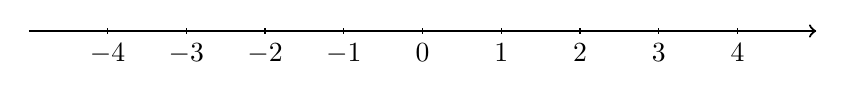
\begin{tikzpicture}
    \draw [->, thick] (-5,0) -- (5,0);
    \foreach \x in {-4,...,4}
        \draw (\x cm, 1pt) -- (\x cm, -1pt) node [anchor=north] {$\x$};
\end{tikzpicture}

\subsubsection{Darstellung}Darstellung von Funktionen mittels Wertetabellen, Graphen und Formeln (Funktionsvorschriften). Oder durch beschreiben, z.B.: \textsl{für jedes $x$ wächst $y$ um 1.5}.

\subsection{Einfache, lineare Funktionen}
\subsubsection{Monotonie}Funktionen können in einem \textbf{Abschnitt} (streng) monoton \textbf{steigend} oder (streng) monoton \textbf{fallend} sein. \\[1em]
\begin{tabularx}{\textwidth}{|rX|}
    \hline
    \textbf{Monoton steigend:}&Eine Funktion verläuft in einem Abschnitt teils horizontal, teils steigend.\\
    \textbf{Streng monoton steigend:}&Eine Funktion steigt in einem Abschnitt durchgehend, wird nie horizontal oder gar fallend.\\
    \textbf{Monoton fallend:}&Eine Funktion verläuft in einem Abschnitt teils horizontal, teils fallend.\\
    \textbf{Streng monoton fallend:}&Eine Funktion fällt in einem Abschnitt durchgehend, wird nie horizontal oder gar steigend.\\
    \hline
\end{tabularx}\\[1em]
Die Funktion kann (streng) monoton \textbf{steigend/fallend} sein, falls sie für alle x steigt oder fällt.

\subsubsection{Proportionalität}Wir sagen $y$ ist (direkt) proportional zu $x$, falls es eine Konstante $a$ gibt, sodass\\
$y=ax,\quad$ $a$ heisst \textsl{Proportionalitätskonstante}.

\subsubsection{Umgekehrt proportionale Funktionen}Beispiel: Die Durchschnittsgeschwindigkeit auf der Strecke $s=50km$ hängt umgekehrt proportional von der dafür benötigten Zeit $t$ ab, $v=\frac{s}{t}$. Heisst soviel, dass auch wenn sich die Strecke ändert, sich zwangsläufig auch die Zeit ändern muss, um die gleiche Durchschnittsgeschwindigkeit $v$ beizubehalten, z.B. $v=\frac{2\times 50km}{2\times t}$.

\subsubsection{Verschiebung und Skalierung von Funktionen}Verschiebt man eine Funktion $y=ax$ um $b$ in $y$-Richtung, erhält man die lineare Funktion $y=ax+b$.

\subsubsection{Differenzenquotient}Der \textbf{Differenzenquotient} von $f$ an der Stelle $x$ ist definiert durch:
\begin{align*}
    \frac{\Delta y}{\Delta x}=\frac{f(x+\Delta x)-f(x)}{\Delta x}
\end{align*}

\subsubsection{Gerade und ungerade Funktionen}
\begin{itemize}
    \item Eine gerade Funktion $f$ ist \textbf{achsensymmetrisch} bezüglich der $y$-Achse und es gilt:\\$f(-x)=f(x),\forall x \in D(f)$
    \item Eine ungerade Funktion $f$ ist \textbf{punktsymmetrisch} bezüglich dem Ursprung und es gilt:\\$f(-x)=-f(x),\forall x \in D(f)$
\end{itemize}
\subsection{Exponentialfunktionen}
\subsubsection{Begriffe}Eine Funktion der $f(x)=a\cdot b^x$ mit $b>0$ und $b\neq 1$ heisst \textbf{Exponentialfunktion}. $a$ heisst \textbf{Anfangswert} und $b$ heisst \textbf{Wachstumsfaktor}. Für Definitions- und Wertebereich gilt: $D(f)=\mathbb{R},\, W(f)=\mathbb{R^+}$


\subsection{Neue aus alten Funktionen}

\subsubsection{Verschiebung und Streckung}

\subsubsection{Zusammengesetzte Funktionen}

\subsection{Logarithmusfunktionen}

\subsection{Potenzfunktionen, Polynome und rationale Funktionen}

\newpage
\section*{Formelsammlung}
\subsection*{Einfache lineare Funktionen}
Lineare Funktion
\begin{align*}
    y=&ax+b \\
    y_2-y_1=&a(x_2-x_1)\\
    a=&\frac{y_2-y_1}{x_2-x_1}=\frac{\Delta y}{\Delta x}
\end{align*}

Differenzenquotient
\begin{align*}
    \frac{\Delta y}{\Delta x}=\frac{f(x+\Delta x)-f(x)}{\Delta x}
\end{align*}

\printindex
\end{document}